%!  pour pdfLatex
\documentclass[a4paper]{article}
%\usepackage[hmargin={1.5cm,1.5cm},vmargin={2.4cm,2.4cm},headheight=13.1pt]{geometry}
\usepackage[a4paper,landscape,twocolumn,
            hmargin=1.8cm,vmargin=2.2cm,headheight=13.1pt]{geometry}

\usepackage[pdftex]{graphicx,color}
\usepackage[pdftex,colorlinks={true},urlcolor={blue},pdfauthor={remy Nicolai}]{hyperref}

\usepackage[T1]{fontenc}
\usepackage[utf8]{inputenc}

\usepackage{lmodern}
\usepackage[frenchb]{babel}

\usepackage{fancyhdr}
\pagestyle{fancy}

\usepackage{floatflt}
\usepackage{maths}

\usepackage{parcolumns}
\setlength{\parindent}{0pt}

\usepackage{caption}
\usepackage{subcaption}

\usepackage{makeidx}

\usepackage[french,ruled,vlined]{algorithm2e}
\SetKwComment{Comment}{\#}{}
\SetKwFor{Tq}{tant que}{}{}
\SetKwFor{Pour}{pour}{}{}
\DontPrintSemicolon
\SetAlgoLined

\usepackage{listings}
\lstset{language=Python,frame=single}
\lstset{literate=
  {á}{{\'a}}1 {é}{{\'e}}1 {í}{{\'i}}1 {ó}{{\'o}}1 {ú}{{\'u}}1
  {Á}{{\'A}}1 {É}{{\'E}}1 {Í}{{\'I}}1 {Ó}{{\'O}}1 {Ú}{{\'U}}1
  {à}{{\`a}}1 {è}{{\`e}}1 {ì}{{\`i}}1 {ò}{{\`o}}1 {ù}{{\`u}}1
  {À}{{\`A}}1 {È}{{\'E}}1 {Ì}{{\`I}}1 {Ò}{{\`O}}1 {Ù}{{\`U}}1
  {ä}{{\"a}}1 {ë}{{\"e}}1 {ï}{{\"i}}1 {ö}{{\"o}}1 {ü}{{\"u}}1
  {Ä}{{\"A}}1 {Ë}{{\"E}}1 {Ï}{{\"I}}1 {Ö}{{\"O}}1 {Ü}{{\"U}}1
  {â}{{\^a}}1 {ê}{{\^e}}1 {î}{{\^i}}1 {ô}{{\^o}}1 {û}{{\^u}}1
  {Â}{{\^A}}1 {Ê}{{\^E}}1 {Î}{{\^I}}1 {Ô}{{\^O}}1 {Û}{{\^U}}1
  {œ}{{\oe}}1 {Œ}{{\OE}}1 {æ}{{\ae}}1 {Æ}{{\AE}}1 {ß}{{\ss}}1
  {ű}{{\H{u}}}1 {Ű}{{\H{U}}}1 {ő}{{\H{o}}}1 {Ő}{{\H{O}}}1
  {ç}{{\c c}}1 {Ç}{{\c C}}1 {ø}{{\o}}1 {å}{{\r a}}1 {Å}{{\r A}}1
  {€}{{\euro}}1 {£}{{\pounds}}1 {«}{{\guillemotleft}}1
  {»}{{\guillemotright}}1 {ñ}{{\~n}}1 {Ñ}{{\~N}}1 {¿}{{?`}}1
}

%pr{\'e}sentation des compteurs de section, ...
\makeatletter
\renewcommand{\thesection}{\Roman{section}.}
\renewcommand{\thesubsection}{\arabic{subsection}.}
\renewcommand{\thesubsubsection}{\arabic{subsubsection}.}
\renewcommand{\labelenumii}{\theenumii.}
\makeatother


\newtheorem*{thm}{Théorème}
\newtheorem{thmn}{Théorème}
\newtheorem*{prop}{Proposition}
\newtheorem{propn}{Proposition}
\newtheorem*{pa}{Présentation axiomatique}
\newtheorem*{propdef}{Proposition - Définition}
\newtheorem*{lem}{Lemme}
\newtheorem{lemn}{Lemme}

\theoremstyle{definition}
\newtheorem*{defi}{Définition}
\newtheorem*{nota}{Notation}
\newtheorem*{exple}{Exemple}
\newtheorem*{exples}{Exemples}


\newenvironment{demo}{\renewcommand{\proofname}{Preuve}\begin{proof}}{\end{proof}}
%\renewcommand{\proofname}{Preuve} doit etre après le begin{document} pour fonctionner

\theoremstyle{remark}
\newtheorem*{rem}{Remarque}
\newtheorem*{rems}{Remarques}

%\usepackage{maths}
%\newcommand{\dbf}{\leftrightarrows}

%En tete et pied de page
\lhead{Informatique}
%\chead{Introduction aux systèmes informatiques}
\rhead{MPSI B Hoche}
\lfoot{\tiny{Cette création est mise à disposition selon le Contrat\\ Paternité-Partage des Conditions Initiales à l'Identique 2.0 France\\ disponible en ligne http://creativecommons.org/licenses/by-sa/2.0/fr/  
} 
\rfoot{\tiny{Rémy Nicolai \jobname \; \today } }
}
\makeindex

%En tete et pied de page
\lhead{Cours IPT}
\chead{Introduction à Scilab et au calcul numérique}
\begin{document}
\section{Introduction à Scilab} 
Ce texte est une introduction à Scilab qui peut vous guider dans la consultation de l'aide en ligne lors de vos premiers travaux.
\subsection{Présentation}
Scilab est un langage de programmation interprété associé à une collection d'algorithmes numériques de calcul scientifique. Il est distribué sous licence libre et un environnement d'utilisation est disponible pour les principaux O.S. à l'adresse \href{http://www.scilab.org}{http://www.scilab.org}.

L'espace de travail (environnement d'utilisation) est constitué de plusieurs fenêtres:
\begin{itemize}
  \item la console pour exécuter des commandes
  \item l'éditeur pour écrire des programmes
  \item les fenêtres graphiques pour afficher des graphiques
  \item le navigateur d'aide
\end{itemize}
La console permet d'exécuter des commandes une après l'autre ce qui est commode pour se familiariser avec le langage puis pour tester des éléments de code. La fenêtre en haut à droite de "Navigateur de variables" est aussi utile pour garder la maîtrise de ce que représentent les noms déjà définis.\newline 
Après l'invite \texttt{-->}, saisir une commande et appuyer sur la touche "Entrée" ou "Retour" du clavier.
\begin{verbatim}
  --> 57/4
  -->1 + 2
\end{verbatim}
Le point du \texttt{3.} du deuxième exemple signifie que ce qui est renvoyé est de type float. En Scilab, tous \emph{les calculs sont numériques}. Les objets mathématiques de base sont donc hors de portée. Scilab ne peut en fournir que des valeurs numériques approchées. Par exemple \texttt{\%e } et \texttt{\%pi} désignent les valeurs approchées des nombres $e$ et $\pi$ et non ces nombres eux mêmes. Les objets du type float en Scilab (qui sont à la base de tous les autres) sont stockées selon la norme IEEE 754 en double précision sur 64 bits. En fait Scilab manipule essentiellement des \emph{matrices}. Dans toute la suite de ce texte, on utilisera abusivement nombre pour float.

En ajoutant un ";" à la fin d'une commande, lors de l'exécution, rien ne s'affiche.

Pour interrompre un programme en cours d'exécution, passer par le menu "Contrôle" de la barre de menu.
\subsection{Obtenir de l'aide}
Le \emph{navigateur d'aide} est le principal outil. On peut l'ouvrir en passant par le "?" de la barre de menu puis "Aide de Scilab" ou bien en tapant simplement sur le "F1" du clavier. Accéder à l'aide par un arbre ou tapant un mot.\newline
On peut aussi ouvrir le navigateur et le placer sur un mot particulier en tapant \texttt{--> help mot} dans la console.

\subsection{L'éditeur}
L'éditeur proposé avec l'environnement est appelé sciNotes. On peut l'ouvrir en utilisant la premiere icone de la barre d'outils ou par Applications>SciNotes de la barre de menus.\newline
L'ergonomie de SciNotes est classique: enregistrement par Fichier>Enregistrer de la barre de menus ou par l'icone de la barre d'outils. Un fichier avec l'extension ".sce" est créé.\newline
Pour exécuter le code contenu dans un fichier, passer par Exécuter de la barre de menus. Plusieurs possibilités sont proposées, qui affichent ou non les commandes dans la console.\newline
Les commentaires sont précédés par "//". En principe une seule commande est placée par ligne. On peut en écrire plusieurs en les séparant par des ";" ou des ",".\newline
Les espaces sont ignorés, la casse (majuscule / minuscule) est significative.

\subsection{Types de données}
\begin{itemize}
  \item "nombres réels" : float
  \item matrices de nombres
  \item booléens \texttt{\%t} ou \texttt{\%T}, \texttt{\%f} ou \texttt{\%F}. Les opérateurs 
  \begin{verbatim}
    &  |  ~  ==  ~=  <>  <  >  <=  >=
  \end{verbatim}
renvoient des valeurs booléennes. Noter que \texttt{~a} est la négation de \texttt{a} et que l'on peut utiliser indifféremment \texttt{~=} ou \texttt{<>}.
Noter que \texttt{\&} est la forme infixe de la fonction préfixe \texttt{and}. Idem pour \texttt{|} et \texttt{or}.
\item Entiers : plusieurs sortes d'entiers en dehors des "entiers flottants".
\item Chaînes de caractères: délimiteurs \texttt{"}.
\end{itemize}

\subsection{Fonctions utiles}
La syntaxe d'appel d'une fonction est classique : nom de la fonction suivie des paramètres entre parenthèses. Les notations des opérations usuelles sont standards : "+", "*", "\textasciicircum" (puissance).\newline
La fonction \texttt{disp} affiche l'évaluation de son argument.\newline
Pour \texttt{x} désignant un nombre complexe,
\begin{itemize}
  \item \texttt{sqrt(x)} : renvoie la racine carrée de partie réelle positive ou nulle. Attention, le \texttt{sqrt} d'un produit n'est pas toujours le produit des \texttt{sqrt}. 
  \item \texttt{exp(x)}, \texttt{abs(x)} : exponentielle ou module.  
\end{itemize}
Pour \texttt{x} désignant un nombre complexe \texttt{int(x)} (troncature), \texttt{floor(x)}, \texttt{ceil(x)}.

\texttt{factorial} , \texttt{sum}, \texttt{prod}, \texttt{gsort} (pour trier).

\texttt{length} , \texttt{size}

\texttt{tic} , \texttt{toc} déclenche et arrête un chronomètre.

\texttt{format} permet de modifier le nombre de chiffres \emph{présentés} dans les résultats (mais le nombre des chiffres \emph{utilisés} reste le même)
Chercher dans la l'aide les détails sur ces fonctions.

\subsection{Matrices}
Dans Scilab, toutes les données sont des matrices. Les nombres (éventuellement complexes mais float) sont des matrices $1\times1$.\newline
Constructeur-délimiteur : les crochets "\texttt{[ ]}" avec des séparateurs "," pour des matrices lignes ou ";" pour des matrices colonnes.
\begin{verbatim}
  disp([1,3,7]) ; disp([1;3;7]); truc = [1,2,[4;8],[77,55,88]];
\end{verbatim}
Noter les deux rôles de ";". L'erreur produite montre qu'il s'agit bien de matrices et non de tableaux.\newline
Examiner l'effet de l'exécution de \texttt{truc = [[1;2],[4;8],[77;55]]} sur la fenêtre de navigateur de variables.\newline
L'opérateur "\texttt{:}" renvoie une matrice ligne de nombres. Plus précisément, si \texttt{a} et \texttt{b} désignent des nombres $a$ et $b$, \texttt{a:b} renvoie la matrice lignes des nombres $x$ tels que $a\leq x \leq b$. Si $b<a$ la matrice vide est renvoyée. On peut introduire un deuxième ":". Le terme du milieu désigne alors l'incrément. Exemple :\texttt{8:-1.1:-5}.

L'itérateur \texttt{for} permet de parcourir une matrice ligne selon la syntaxe
\begin{verbatim}
  // matrice est le nom d'une matrice
  for truc = matrice
    // truc désigne l'élément (valeur) courant de la matrice 
    instructions;
  end
\end{verbatim}
En particulier, pour faire varier un compteur \texttt{i} en l'incrémentant de 1 entre deux entiers désignés par \texttt{a} et \texttt{b}, utiliser 
\begin{verbatim}
  for i = a:b instructions; end
\end{verbatim}
Les parenthèses permettent d'accéder aux valeurs d'une matrice et de les modifier. Si \texttt{nomv} est le nom d'une variable, Scilab considère toujours que c'est le nom d'une matrice. En conséquence, si \texttt{i} désigne un entier, le langage évalue \texttt{nomv(i)} comme la ieme valeur de la matrice en renvoyant une erreur d'index si \texttt{i} ne désigne pas un indice acceptable.
\begin{verbatim}
  u = [1,2,3,4,7,8]; disp(u(4)); disp(u(9));  
  u = [1;2;3;4;7;8]; disp(u(4)); disp(u(9)); 
  u = [[1,2];[3,4];[7,8]]]; disp(u(1)); disp(u(2));
  disp(u(3));disp(u(4)); disp(u(9));  
\end{verbatim}
Si \texttt{nomv(i)} est à gauche d'un signe \texttt{=} et si l'expression à droite est évaluée à un type compatible avec \texttt{nomv}, la matrice est étendue par des valeurs nulles jusqu'à l'indice \texttt{i}.
\begin{verbatim}
  u = 4:10 ; u(15) = 17.5; disp(u)
\end{verbatim}
Attention le premier indice d'une matrice est $1$ et non pas $0$.

\subsection{Programmation}
\subsubsection{Assignations - Noms}
Scilab est un langage non typé c'est à dire que les noms ne doivent pas être déclarés et qu'ils peuvent désigner des objets de différents types. 
Tout mot qui n'est pas un élément du langage Scilab lui même ou déjà introduit dans le code est le \emph{nom} d'une fonction ou d'un objet non exécutable de l'un des types que peut gérer Scilab. Il faut bien penser que Scilab est un langage de calcul numérique et qu'il ne peut manipuler que des objets construits à partir du type "double" de la norme IEEE 754.\newline
Pour sa première apparition, un nouveau mot doit être associé au signe "=".\newline
Pour assigner à une variable, placer directement le mot à gauche de "=". Il désigne alors le résultat de l'évaluation de l'expression qui est placée à droite.
\begin{verbatim}
   truc = 2*%pi; exp(truc)
\end{verbatim}
Dans la console, si le résultat d'un calcul n'est pas assigné explicitement à une variable, il l'est par défaut à la variable désignée par \texttt{ans}. (answer)\newline
La syntaxe de définition d'une fonction est plus compliquée. Elle utilise les éléments de langage \texttt{function} et \texttt{endfunction} et le nom de la fonction doit bizarrement être placé à \emph{droite} de l'égalité:
\begin{verbatim}
  function sortie = nom_de_fonction(entree)
       instructions assignant la valeur voulue à sortie;
  endfunction
\end{verbatim}
Les noms \texttt{sortie} et \texttt{entree} sont locaux au segment de code entre \texttt{function} et \texttt{endfunction}. Ils peuvent être remplacés par n'importe quels autres mots qui ne sont pas des éléments du langage.

Nom et parenthèses. Un nom peut toujours être suivi de parenthèses, elles n'ont pas la même signification suivant que le mot désigne une fonction ou une variable.  Si \texttt{nomf} est le nom d'une fonction, \texttt{nomf(truc)} est l'appel usuel de la fonction qui peut éventuellement déclencher une erreur. Une commande \texttt{nomf(truc) = 17.2} va produire une erreur. En revanche, pour une variable (qui est une matrice par défaut) \texttt{nomv(truc)} désigne la valeur d'indice \texttt{truc} de la matrice si cela a du sens.


\subsubsection{Structures de contrôle}
La syntaxe basique du branchement \texttt{if} est standard:
\begin{verbatim}
  if ( cond ) then
    instructions
  else
    autres intructions
  end
\end{verbatim}
où \texttt{cond} s'évalue en booléen. Le \texttt{else} et le segment de code qui suit sont facultatifs. On peut aussi introduire des segments de code avec des \texttt{elseif} entre les segments principaux.

Le branchement \texttt{select} permet de combiner proprement plusieurs \texttt{if} pour diriger vers plusieurs possibilités. Voir l'aide.

La syntaxe de la boucle \texttt{while} est basique.
\begin{verbatim}
  while ( cond )
    instructions
  end
\end{verbatim}
où \texttt{cond} s'évalue en booléen. Comme en Python, \texttt{for} est plutôt un itérateur (des valeurs d'une matrice) qu'une véritable structure de contrôle.


\section{Problématique du calcul numérique}
\subsection{Certains problèmes ne sont pas numériques.}
L'ensemble des float normalisés est impuissant à rendre compte de certaines situations mathématiques. Ce qui suit en est un exemple.\newline
On considère des suites de nombres réels définies par une relation de récurrence d'ordre $2$ et deux valeurs initiales.
\begin{displaymath}
  u_1>0,\; u_2>0,\;
  \forall n>2:\;
  u_{n}= 111 - \frac{1130}{u_{n-1}} + \frac{3000}{u_{n-1}u_{n-2}}
\end{displaymath}
\subsubsection{Approche numérique avec Scilab}
Ici encore \emph{numérique} signifie dans le sous-ensemble normalisé des décimaux. La syntaxe comme matrice est très confortable pour calculer de telles suites
\begin{verbatim}
  n = 40; u(1) = 2; u(2) = 3
  for i = 3:n
    u(i) = 111 - 1130/u(i-1) + 3000/(u(i-1)*u(i-2))
    disp(u(i))
  end
\end{verbatim}
S'il ne s'agit que de calculer le terme d'indice \texttt{n}, on peut économiser de l'espace en ne gardant que les valeurs utiles à la continuation du calcul.
\begin{verbatim}
  n = 40; u = 2; uu = 3
  for i = 3:n
    uuu = 111 - 1130/uu + 3000/(uu*u)
    u = uu
    uu = uuu
  end
  disp(uu)
\end{verbatim}
Pour les conditions initiales proposées, il semble que la suite converge vers $100$. Si on refait les calculs avec les valeurs initiales $(\frac{11}{2},\frac{61}{11})$, on constate encore une convergence numérique vers $100$.

\subsubsection{Approche rationnelle avec SymPy}
Cette fois \emph{rationnelle} signifie que l'on travaille dans $\Q$ avec la bibliothèque de calcul formel sympy pour Python. Il est bien clair que si les valeurs initiales sont rationnelles, toutes les valeurs définies de la suite le sont également. On exécute le code Python suivant. 
\begin{verbatim}
n = 40
u = 11./2.
uu = 61./11.
print(u,uu)
for i in range(3,n):
    uuu = 111 - 1130/uu + 3000/(uu*u)
    u = uu
    uu = uuu
    print(uu)

import sympy
u = sympy.Rational(11,2)
uu = sympy.Rational(61,11)
print(u,uu)
for i in range(3,n):
    uuu = 111 - 1130/uu + 3000/(uu*u)
    u = uu
    uu = uuu
    print(uu, uu.evalf())  
\end{verbatim}
Que peut-on en conclure?
\subsubsection{Approche mathématique avec Scilab et SymPy}
Si une suite $(u_n)_{n\in \N^*}$ converge, sa limite est une racine du polynôme
\begin{displaymath}
  X^3 - 111X^2+1130X-3000
\end{displaymath}
On peut évaluer numériquement les racines avec Scilab en exécutant
\begin{verbatim}
P = poly([-3000,1130,-111,1],"X","coeff")
disp(P)
racines = roots(P)  
\end{verbatim}
Il semble que les racines soient $5$, $6$ et $100$ mais le calcul numérique ne le prouve pas. Pour s'en convaincre, on peut évaluer numériquement un nombre trouvé par Ramanujan:
\begin{verbatim}
format(25) // pour afficher toutes les décimales possibles
exp(%pi*sqrt(163))  
\end{verbatim}
qui n'est évidemment pas entier. En revanche, développer le polynôme
\begin{displaymath}
  (X-5)(X-6)(X-100)
\end{displaymath}
constitue bien une preuve. On peut le faire à la main ou avec SymPy.
\begin{verbatim}
X = sympy.symbols('X')
P = (X-5)*(X-6)*(X-100)
P = sympy.expand(P)
print(P)
\end{verbatim}
Notons $\mathcal{P}$ le plan $\R^2$ privé des deux axes de coordonnées. On peut définir une fonction $F$ de $\mathcal{P}$ dans $\R^2$ par:
\begin{displaymath}
  (x,y)\mapsto (y, 111 - \frac{1130}{y} + \frac{3000}{xy})
\end{displaymath}
Les suites de nombres sont alors associées à des suites de points:
\begin{displaymath}
  P_1 = (u_1,u_2),\; \forall n\geq 2, P_n = (u_n,u_{n+1}) = F(P_{n-1})
\end{displaymath}
La fonction $F$ a trois points fixes : $A=(5,5)$, $B=(6,6)$, $C=(100,100)$. Les expérimentations numériques menées avec Scilab semblent montrer que $C$ est stable et $A$, $B$ instables. La situation est mathématiquement un peu plus compliquée. Il existe en fait une courbe $\Gamma$ (contenant $A$ et $B$ mais pas $C$) et globalement stable c'est à dire que $M\in \Gamma$ entraîne $f(M)\in \Gamma$. Lorsque le point initial est sur cette courbe tous les points de la suite restent sur cette courbe et convergent vers $B$. Lorsque le point initial n'est pas sur la courbe, la suite de points converge vers $C$. L'équation de la courbe est à coefficients entiers donc en calcul formel avec un point initial sur la courbe, la convergence mathématique se réalise bien. En revanche, en calcul numérique, à cause des erreurs d'arrondi les points sortent de la courbe et sont capturés par le bassin d'attraction de $C$.\newline
Avec une bibliothèque de calcul formel, on pourrait trouver l'équation de la courbe stable et prouver sa stabilité mais ce n'est pas l'objet de cette introduction. En restant numérique, on peut avoir une idée de courbe en considérant tous les points dont les abscisses sont entre $1.1$ et $10$. Pour chaque point, on forme la suite dont les valeurs initiales sont les coordonnées du point. On trace le point seulement si le nombre d'itérations nécessaire pour être proche de $100$ est supérieur à une valeur donnée. On propose le code suivant en Python
\begin{verbatim}
import matplotlib.pyplot as plt

def bonindice(u,uu):
  eps = 1.0E-5
  n = 40
  i = 0
  while  abs(uu-100) > eps and i < n:
    uuu = 111. - 1130./uu + 3000./(uu*u)
    u = uu
    uu = uuu
    i += 1
  return i

xmin = 0.1
xmax = 10.
ymin = 0.1
ymax = 10
nx = 2000
ny = 2000
pasx = (xmax-xmin)/nx
pasy = (ymax-ymin)/ny
Lx = [xmin + i*pasx for i in range(0,nx)]
Ly = [ymin + i*pasy for i in range(0,ny)]

for x in Lx:
    for y in Ly:
        if bonindice(x,y) > 11:
            print(x,y,bonindice(x,y))
            plt.plot([x],[y],'.r')

plt.show()  
\end{verbatim}
qui permet de tracer la courbe.
\begin{figure}[h]
  \centering
  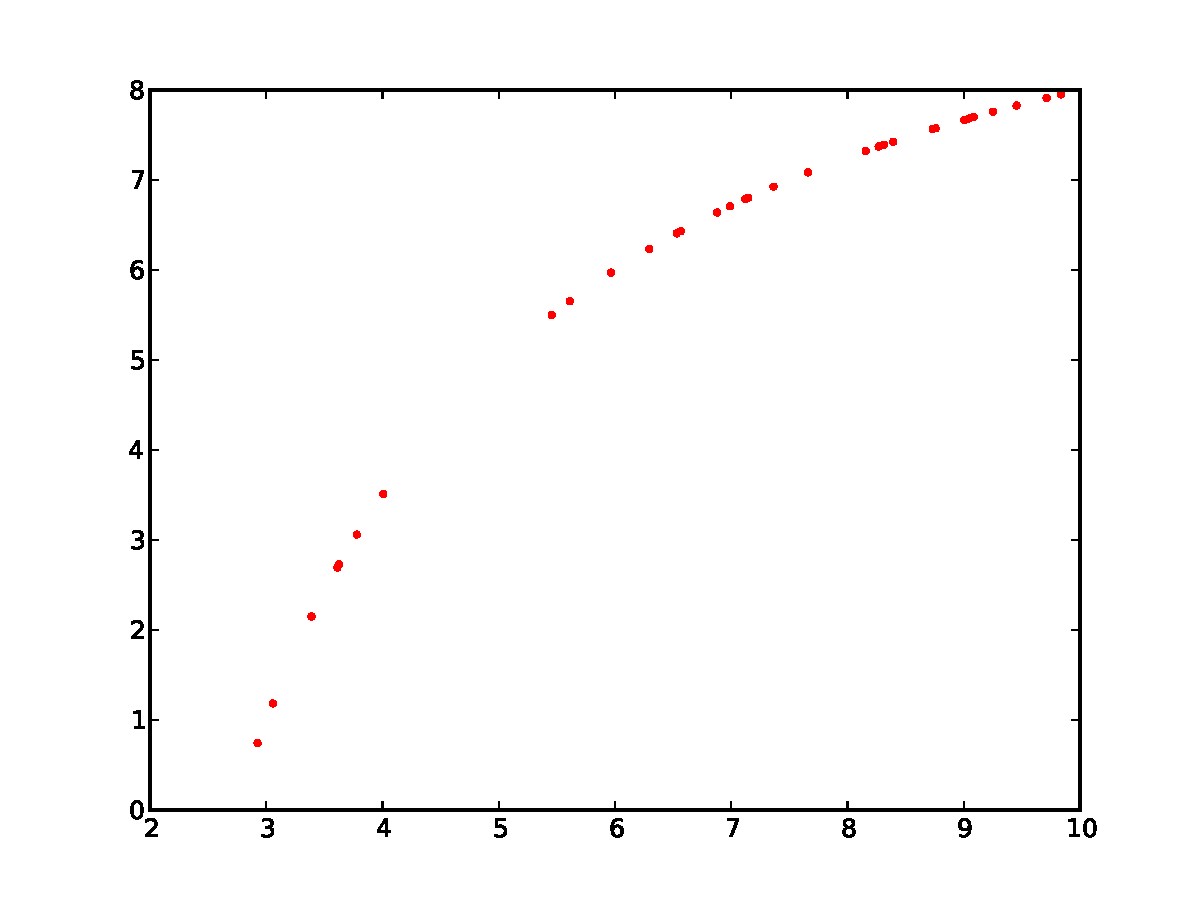
\includegraphics[width=8cm]{./introcalcnum_1_fig.pdf}
  % introcalcnum_1.pdf: 576x432 pixel, 72dpi, 20.32x15.24 cm, bb=0 0 576 432
  \caption{Courbe globalement stable}
  \label{fig:introcalcnum_1}
\end{figure}
Implémentation en Scilab du tracé de la même courbe
\begin{verbatim}
function i = bonindice(u,uu)
  eps = 10^(-5)
  nmax = 40
  i = 0
  while ( abs(uu - 100)> eps & i < nmax)
    uuu = 111 - 1130/uu + 3000/(uu*u)
    u = uu
    uu = uuu
    i = i+1
  end
endfunction
xmin = 2; xmax = 10.; ymin = 2. ; ymax = 10;
pasx = 1/88; pasy = 1/88;
Lx = xmin:pasx:xmax; Ly = ymin:pasy:ymax;
i = 1;
for x = Lx;
    for y = Ly;
        p = bonindice(x,y);
        if ( p > 11) then
            xOK(i) = x;
            yOK(i) = y;
            i = i+1;
        end
    end
end
plot(xOK,yOK,'.')
\end{verbatim}
\end{document}